




%%
\begin{figure}[t]
\centering
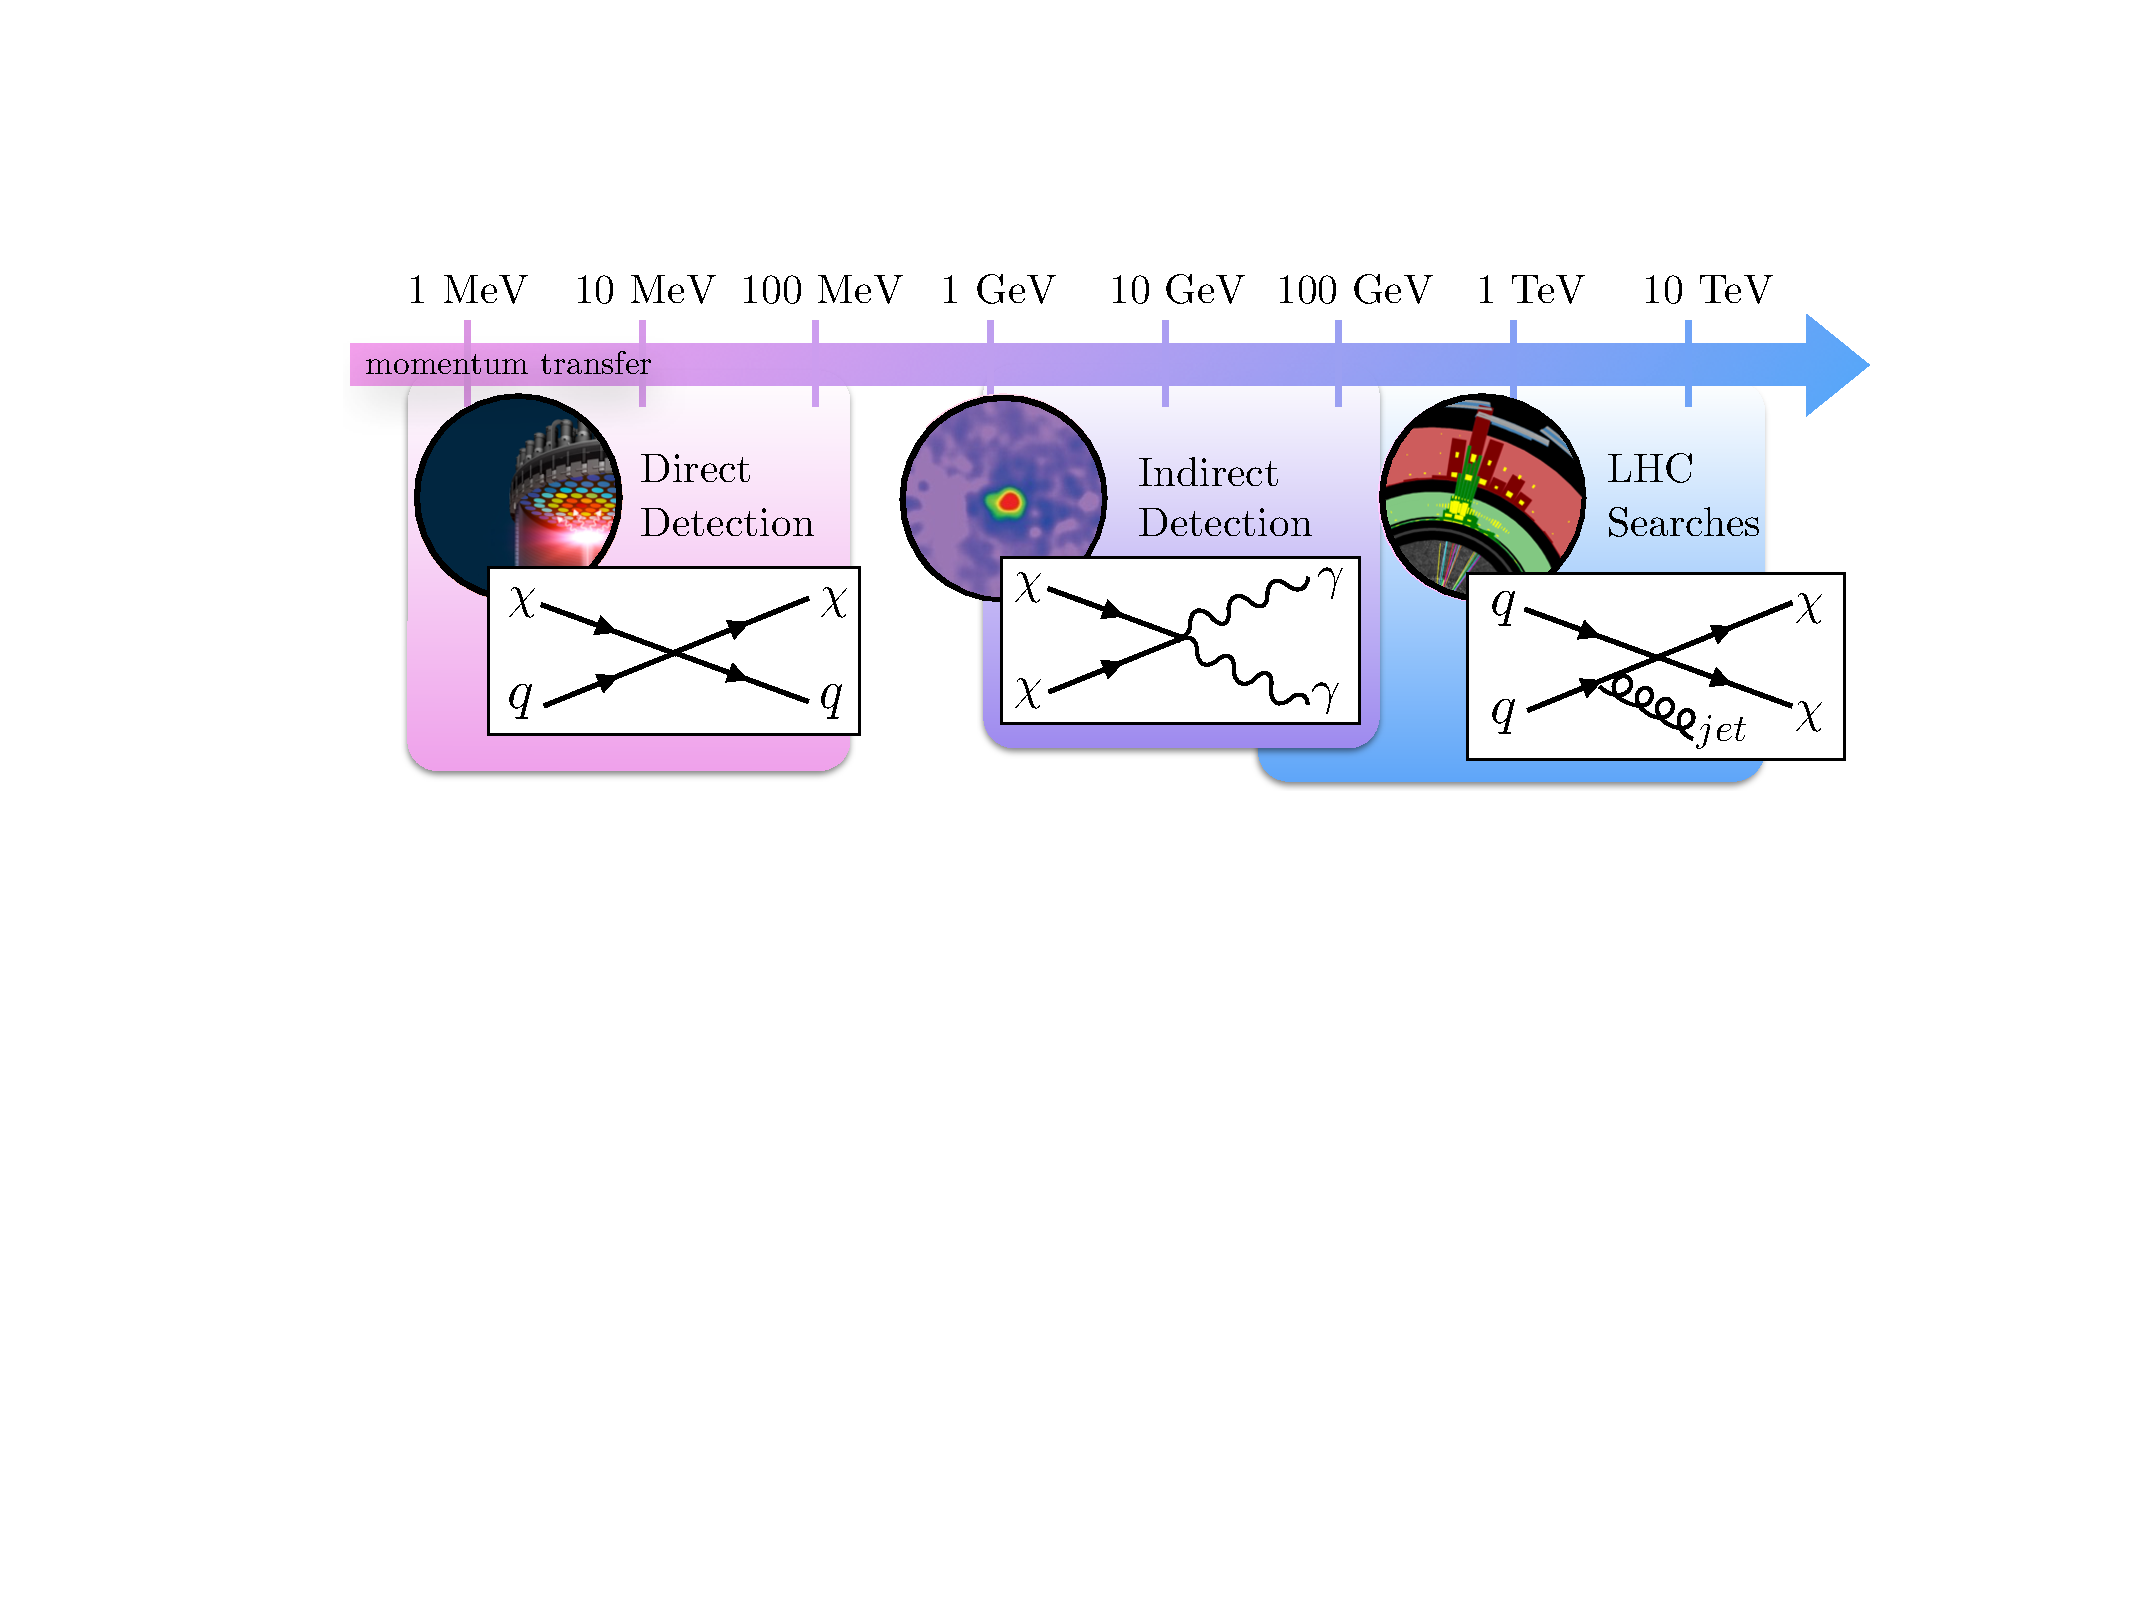
\includegraphics[width=.95\textwidth]{figures/mmt}
\caption{\label{fig:momentumtransfer} Range of momenta probed in Direct Detection experiments, Indirect Detection experiments and LHC searches for weak scale Dark Matter candidates. }
\end{figure}
%%

\subsection{Evolution of theories for Dark Matter searches at colliders} For two of the three Dark Matter search strategies 
-direct and indirect detection- experimental results are presented in terms of effective field theories (EFTs). The operators in these EFTs are build from SM fermions and Dark Matter fields, 
%and one distinguishes different operator structures
\begin{align}\label{eq:EFT}
\mathcal{L}_\text{EFT}= \sum_{f=u, d, \ell} \,\left(\frac{C_{1}^f}{\Lambda^2} \bar f f \bar \chi \chi+ \frac{C^f_{2}}{\Lambda^2}\bar  f f \bar \chi \gamma^5\chi +\frac{C_{3}^f }{\Lambda^2}\bar  f \gamma^5 f \bar \chi \chi +\frac{C_{4}^f}{\Lambda^2} \bar  f \gamma^5 f \bar \chi\gamma^5 \chi \,+\ldots \right) \,,
\end{align}
where $\chi$ denotes a Dirac fermion DM candidate and the sum over $f=u,d,\ell$ extends over SM quarks and leptons. 
The EFT is fully described by the parameters 
\begin{align}\label{eq:EFTparams}
\big\{ m_\chi\,,\,\,\Lambda ,\,\, C_i^f\big\} \,,
\end{align}
where $m_\chi$ is the mass of the DM candidate.
This ansatz is justified for the small momentum transfer $q^2\ll \Lambda^2$ in DM-nucleon scattering (set by the non-relativistic velocities of DM in the halo) and in DM annihilation (set by the mass of the annihilating DM candidate), illustrated in Fig.~\ref{fig:momentumtransfer}. Early papers on DM searches at colliders refer to these EFTs to quantify 
the reach of the LHC in the parameter space defined by \eqref{eq:EFTparams}  \cite{Beltran:2010ww, Fox:2011pm,Goodman:2010ku}. The momentum transfer accessible at the LHC is larger than the suppression scale 
$\Lambda \ll q^2_\text{LHC}$ for many theories of DM. 
In this case, the mediator of the interaction between the dark sector and the SM can be resonantly produced and 
predictions derived from the EFT framework are bound to fail \cite{}. The kinematics   
of on-shell propagators can be captured in simplified models, which aim to represent a large number of extensions 
of the SM, while keeping only the degrees of freedom relevant for LHC phenomenology. In the case of a pseudoscalar mediator the corresponding interactions between DM, SM fermions and the mediator $a$ read
\begin{align}\label{eq:simp}
\mathcal{L}_\text{simp}=-i\,g_\chi a\bar \chi \gamma_5 \chi -i a \sum_i \left(g_u y_i^u \bar u_i \gamma_5 u_i + g_d y_i^d \bar d_i \gamma_5 d_i + g_u\ell y_i^\ell \bar \ell_i \gamma_5 \ell_i  \right) \,,
\end{align}
in which $i$ is a flavour index. In addition, there is the scalar potential including a potential Higgs portal 
\begin{align}\label{eq:VaH}
V(H, a)=\frac{1}{2}m_a^2 a^2+b_{a} a\,H^\dagger H +\lambda_{Ha} a^2H^\dagger H + \lambda a^4\,.
\end{align}
The Higgs portal is generally considered irrelevant, otherwise there are constraints from Higgs coupling strength measurements and of the Higgs CP property stronger than all limits from searches for DM at the LHC \cite{}. The quartic couplings in \eqref{eq:VaH} are not relevant for collider searches for DM.
This simplified model is therefore fully described by the parameters 
\begin{align}
\big\{ m_\chi, \,\, m_a\,,\,\, g_\chi\,, \,\, g_u\,,\,\,g_d\,,\,\, g_\ell \big\}\,,
\end{align}
and
matches to the EFT \eqref{eq:EFT} with $C^f_4/\Lambda^2 = g_\chi g_f y_f  /m_a^2$ and $C_i^f=0$ for all other Wilson coefficients, but retains the full momentum dependence of the pseudoscalar propagator.  The operators in both $\mathcal{L}_\text{EFT}$ and $\mathcal{L}_\text{simp}$ violate gauge invariance, because of the chiral SM fermions. In the case of the EFT this suggests the scaling of the Wilson coefficients $C_i^f= c_i^f m_{f_i}/\Lambda$ \cite{}, whereas for the simplified model restoring gauge invariance requires the embedding of the mediator $a$ into an electroweak multiplet. The absence of gauge invariance leads to unitarity violating amplitudes. For example on the left of Fig.~\ref{fig:diagrams}, we show the diagram contributing to the amplitude for the production of the pseudoscalar mediator in association with a $Z$-boson, which diverges with the center-of-mass energy $\mathcal{M}(pp\to Z a) \propto \log^2(s)$ in the simplified model, signaling the omission of additional diagrams. Since this divergence is only logarithmic, the simplified model does not break down for the energies accessible at the LHC \cite{}. More importantly, the additional degrees of freedom necessary to unitarize the amplitudes cannot be arbitrarily heavy and change the phenomenology of the simplified model significantly. For example, the $pp\to Z a$ cross section can be made finite by the exchange an additional scalar $H$ with a coupling to $a$ and $Z$, and the corresponding diagram is shown on the right of Fig.~\ref{fig:diagrams}. Since resonant production is strongly enhanced compared to initial state radiation, the hierarchy of initial state mono-X signals, mono-jet $>$ mono-photon $>$ mono-$Z$ $>$ mono-Higgs, can be turned upside-down with different kinematics requiring adapted experimental search strategies. The embedding of the pseudoscalar mediator model \eqref{eq:simp} is not unique. Both the mediator and the DM can be embedded in different electroweak multiplets, resulting in additional model-dependent and model-independent signals \cite{}. In this whitepaper, we consider the simplest embedding with a single SM-singlet DM candidate, which captures the maximal number of interesting signatures.     


%%
\begin{figure}
\centering
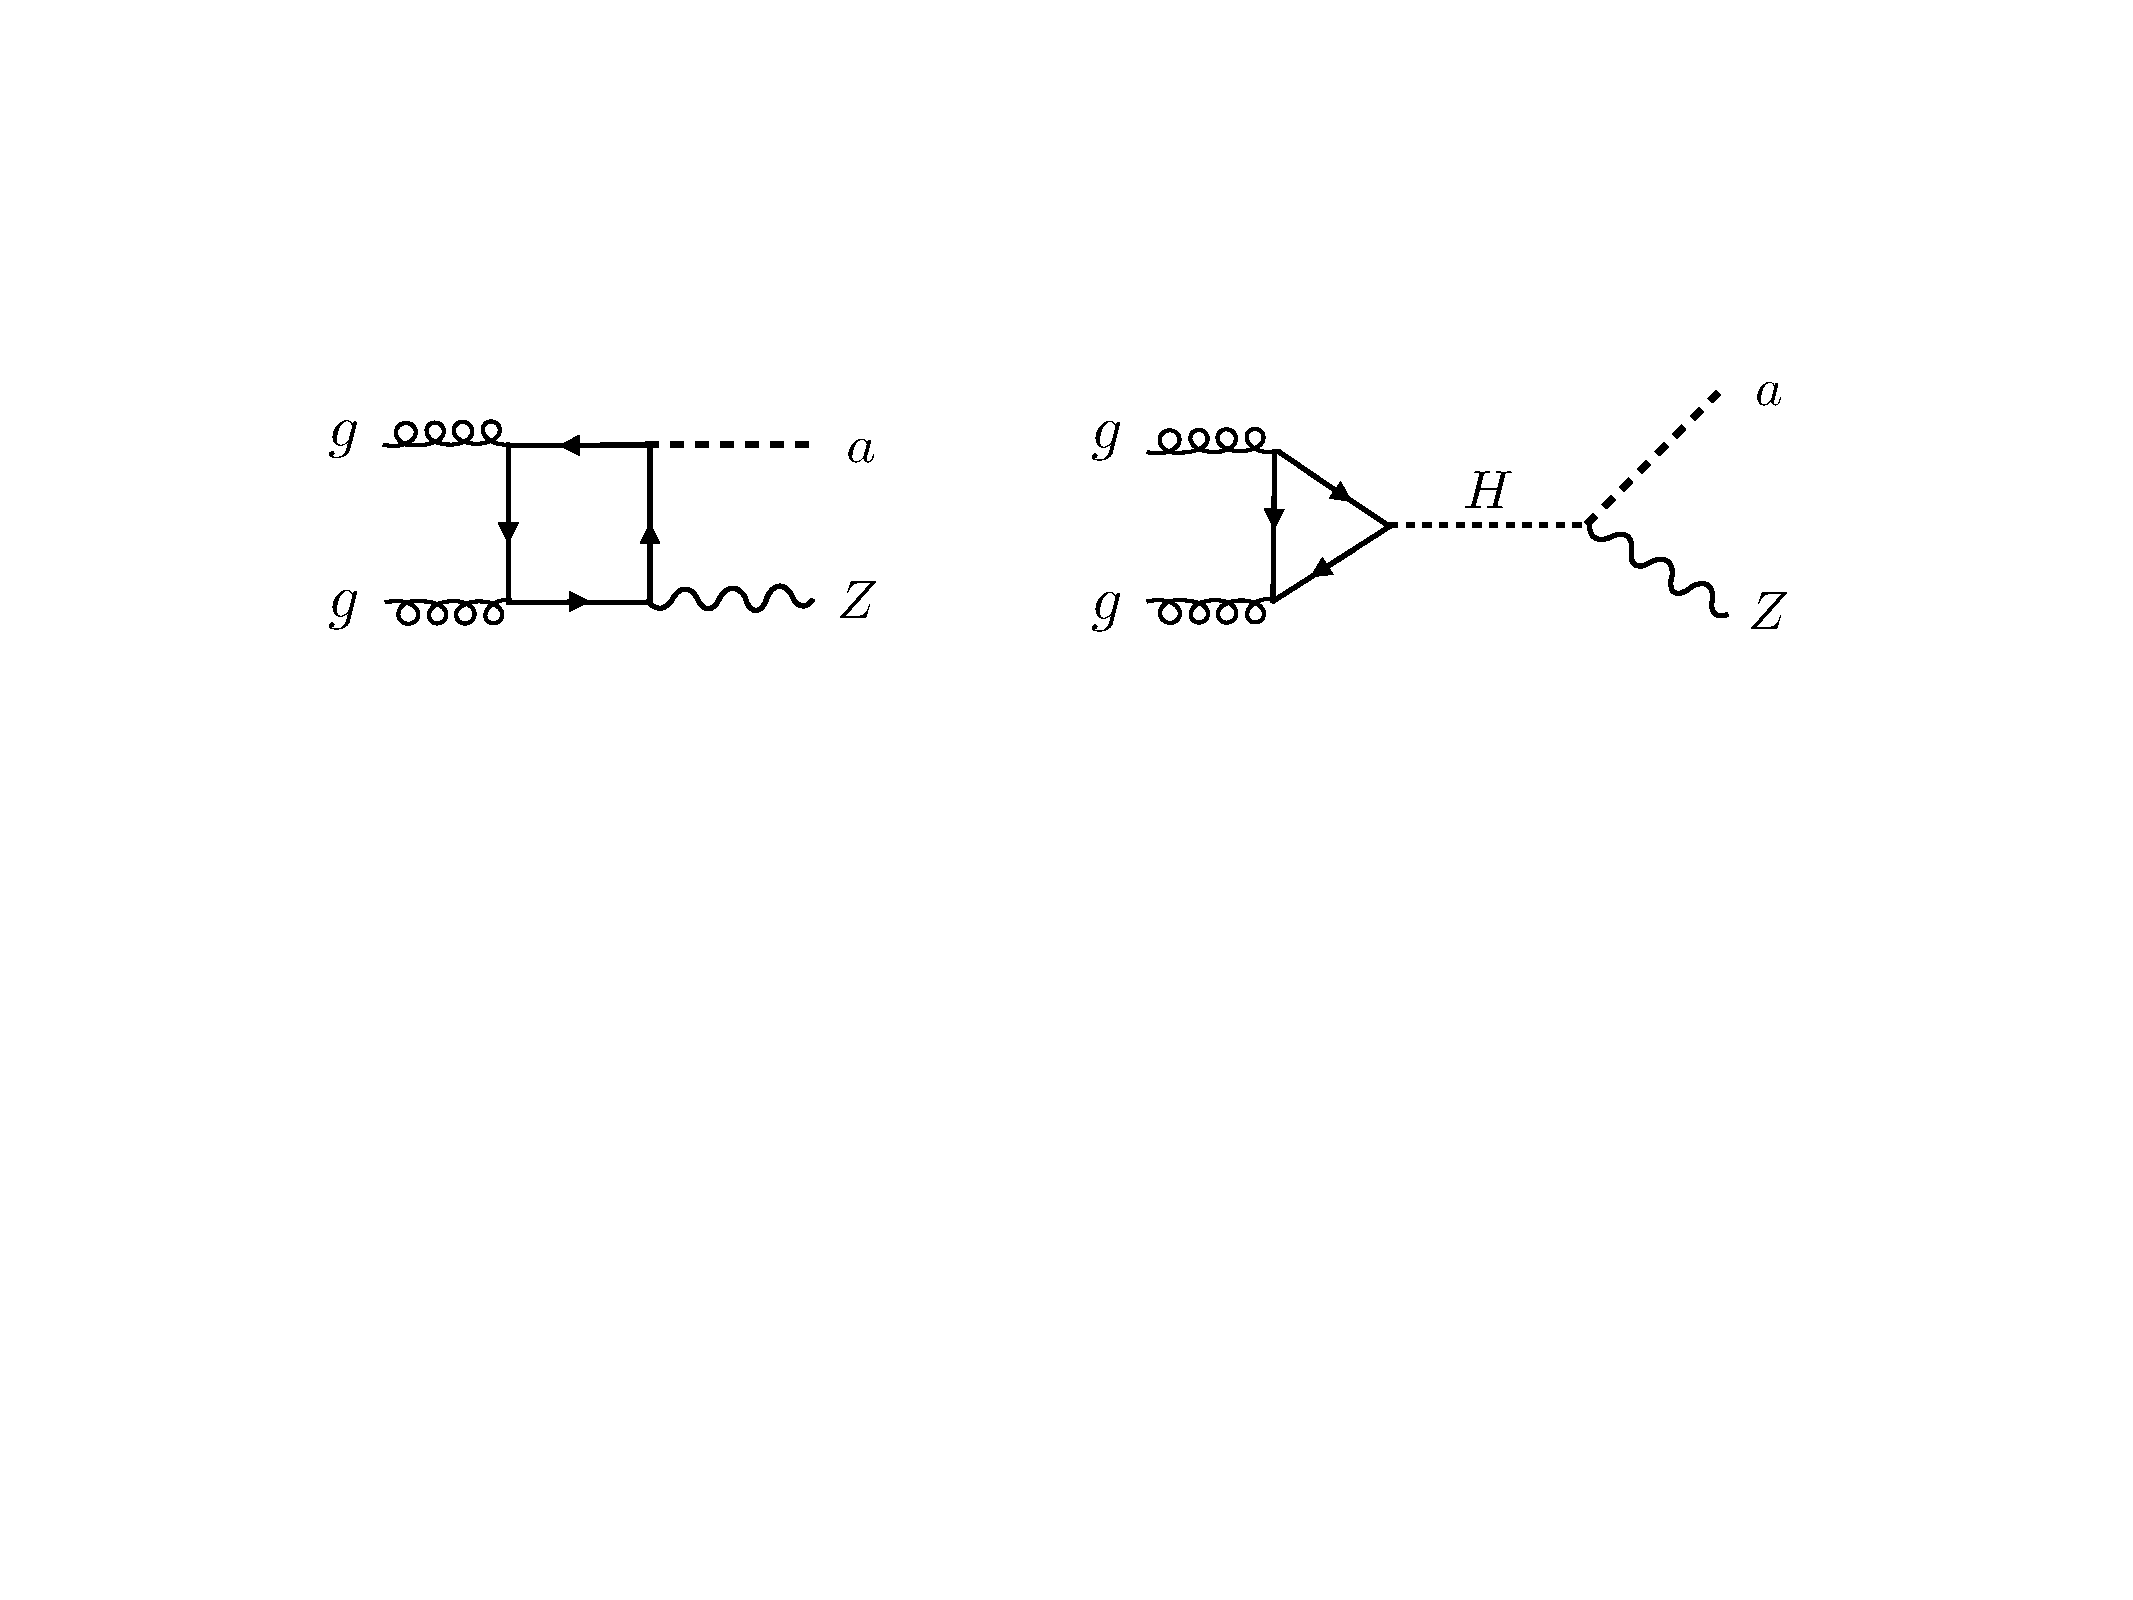
\includegraphics[width=.8\textwidth]{figures/diagrams}
\caption{\label{fig:diagrams} Feynman diagrams contributing to $\sigma(pp \to a Z)$ in the simplified model with a pseudoscalar singlet mediator $a$ (left) and in the 2HDM+a model (right). }
\end{figure}
%%
		

